\section{ Ưu điểm của việc sử dụng Java trong lập trình Android}
    \begin{flushleft}
        \hspace*{0.8cm}Java là một trong những ngôn ngữ lập trình lâu đời và phổ biến nhất trên thế giới. Việc sử dụng Java trong lập trình Android giúp lập trình viên dễ dàng tiếp cận với nguồn tài nguyên phong phú từ tài liệu học tập, ví dụ thực tế đến sự hỗ trợ từ cộng đồng. Java sử dụng hệ thống kiểu dữ liệu chặt chẽ (strongly typed), giúp phát hiện lỗi cú pháp và logic ngay trong quá trình biên dịch. Điều này làm tăng độ an toàn của chương trình và giảm thiểu nguy cơ phát sinh lỗi trong quá trình thực thi.\\
        \hspace*{0.8cm}Một trong những triết lý cốt lõi của Java là “Write once, run anywhere” – nghĩa là mã nguồn chỉ cần viết một lần và có thể chạy trên nhiều nền tảng khác nhau mà không cần chỉnh sửa. Điều này có được là nhờ Java chạy trên máy ảo JVM, giúp mã được biên dịch thành bytecode độc lập với hệ điều hành. Khi lập trình Android bằng Java, điều này đồng nghĩa với việc bạn có thể dễ dàng tái sử dụng phần lớn mã nguồn cho các ứng dụng chạy trên nền tảng khác như desktop hoặc server-side Java.\\
        \hspace*{0.8cm}Hệ sinh thái phát triển rất phong phú với hàng loạt công cụ và thư viện hỗ trợ mạnh mẽ, tiêu biểu như Android Studio – môi trường phát triển chính thức cho Android. Ngoài ra, Gradle giúp tự động hóa quá trình build, còn hàng nghìn thư viện mã nguồn mở khác có thể giúp giảm đáng kể thời gian và công sức viết mã. Hơn nữa, cộng đồng lập trình viên Java rất đông đảo và hoạt động tích cực, giúp bạn dễ dàng tìm được câu trả lời cho các vấn đề kỹ thuật trên các diễn đàn như Stack Overflow, GitHub, hay cộng đồng Google Developer.\\
        \hspace*{0.8cm}Java hỗ trợ cơ chế quản lý bộ nhớ tự động thông qua trình thu gom rác (Garbage Collector). Thay vì phải tự giải phóng bộ nhớ như trong C hoặc C++, lập trình viên Java không cần lo lắng về việc quản lý tài nguyên thủ công. Trình thu gom rác sẽ tự động theo dõi và thu hồi vùng nhớ không còn được sử dụng, giúp ngăn ngừa các lỗi phổ biến như rò rỉ bộ nhớ (memory leak) và tăng độ ổn định của ứng dụng, nhất là trong môi trường như Android – nơi tài nguyên hệ thống bị giới hạn\cite{java-tutorial}.\\
    
        \begin{figure}[H] 
            \centering
            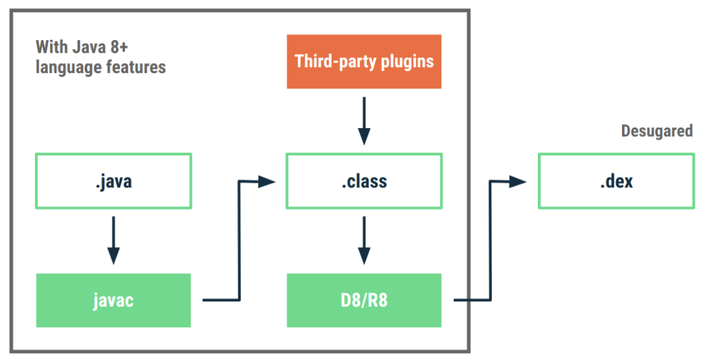
\includegraphics[width=0.8\textwidth]{images/javainandroid.png}
            \caption{Hỗ trợ tính năng ngôn ngữ Java 8 bằng cách desugar biến đổi mã byte.}
            \label{fig:android}
        \end{figure}
        \hspace*{0.8cm}Trình bổ trợ Android cho Gradle cung cấp khả năng hỗ trợ tích hợp để sử dụng một số tính năng ngôn ngữ Java 8 cùng các thư viện bên thứ ba sử dụng những tính năng đó. Chuỗi công cụ mặc định triển khai các tính năng ngôn ngữ mới bằng cách thực hiện các biến đổi mã byte (được gọi là desugar) như một phần của quá trình biên dịch các tệp lớp D8/R8 thành mã DEX, như minh hoạ trong hình\cite{java8}.
    \end{flushleft}

